\chapter{Introduction}

In this thesis, I want to generate a conceptual space for the domain of university courses, automatically created in a data-driven way from their descriptions.

\section{Reading Instructions}

Throughout this thesis we'll use the "we" als \emph{Pluralis Auctoris}, signifying objectivity in science. This does not mean that anyone but the author of this thesis contributed to it. TODO: see how rüdiger \todoparagraph{said that in his acknowledgements} \url{https://www.rki.de/EN/Content/infections/epidemiology/signals/projects/Optimization_Outbreak_Detection_MasterThesis_Busche_2019.pdf?__blob=publicationFile}

\paragraph*{Document Structure}
\todoparagraph{
	Chapter 1 is Intro, with motivations etc. 
	Chapter 2 is Background, explaining the the required concepts - what are conceptual spaces generally, how does the base algorithm work, what kinds of algorithms occur in it. I am explaining the rquired algorithm before the main algo such that I can rely on definitions there.
	Chapter 3 is then methods. Dataset, algorithm, architecture. 
	4 results, 5 conclusion, that's it.
}

\paragraph*{Digital Version}

\todoparagraph{If you're not reading the digital version, I highly recommend it}. The digital version of the document is highly hyperlinked (all glossary entries are linked, you can jump forward and back for sections and citations and references, lists that are detailed later are also forward and backward linked, etc). There is a version with colored links, which I recommend if you're reading digitally. Further, there are many plots in later sections. Unfortunately, a PDF is static so three-dimensional plots are not very obvious. Because of that, sometimes only 2D-Versions are printed here and the 3D-version only referenced. It is highly recommended to follow these links, as they refer interactive plots which can not only be twisted and turned to truly understand them, but also show much additional information that cannot be statically shown, such as detailed information about the respective entities of a scatterplot on mouse-over.


\paragraph*{Regarding Terminology}

Throughout this thesis, many abbreviations, symbols and technical terms will be used. \todoparagraph{I hope that all of that cannot be exptected to be known by the reader are defined. At the end of this thesis there is a} \nameref{sec:glossary} \todoparagraph{with the subsections yadda yadda. If you are reading this document digitally, all occurrences of the terms described there should be a hyperlink (as are all section, table, figure, etc references). If you don't have the version with colored hyperlinks, you can download it here:} \url{https://nightly.link/cstenkamp/MastersThesisText/workflows/create_pdf_artifact/master/Thesis.zip}

\section{Motivation}

\subsection{Course Recommendation}

This thesis explores a novel method to generate explainable recommendations for university-courses and other educational resources. The results will eventually be incorporated into the \emph{Siddata}-platform, helping students to find courses that fit their interests.

\subsubsection*{Overwhelming amounts of resources}

The university landscape has changed drastically in recent years. In 1999, the \textit{Bologna declaration} was signed by the 29 countries of the the \textit{European Higher Education Area} (now 45), reforming their education systems to allow for international compatibility. While before 1999 there were between 70 and 180 different elementary studies \cite{Schroder2015} in Germany, that number had risen to 2554 in 2003,\footnote{\url{https://www.che.de/download/im_blickpunkt_ausdifferenzierung_studiengaenge-pdf/?wpdmdl=10620&refresh=624af74f6f7921649080143}} had become more than 5000 in 2008 and currently (winter semester 2020/2021) peaks at 9168 unique courses of study.\footnote{\url{https://www.hrk.de/fileadmin/redaktion/hrk/02-Dokumente/02-03-Studium/02-03-01-Studium-Studienreform/HRK_Statistik_BA_MA_UEbrige_WiSe_2020_21_finale.pdf}, page 10 \label{fnote:degreenums}} The number of subjects in total has almost doubled in the past thirteen years, from 11\,265 in 2007 to 20\,359 in 2020.\footnoteref{fnote:degreenums} According to the German \textit{Centrum für Hochschulentwicklung}, nowadays only 18.7\% of degrees are \textit{classical}, \ie tailored to a specific subject such as \textit{Physics}, the rest fall unter the categories hybrid, interdisciplinary or topic-focused.\footnote{\url{https://www.che.de/wp-content/uploads/upload/Im_Blickpunkt_Die_Vielfalt_der_Studiengaenge_2017.pdf}}

Where before there was a rigid schedule of mandatory courses, modern courses of studies are becoming increasingly modular, allowing students to draw up individual educational plans composed of a wide selection of courses.\footnote{\url{https://www.pedocs.de/volltexte/2008/285/pdf/heft98.pdf}} Due to globalisation and the introduction of the \emph{European Credit Transfer System}, the selection of courses for this may span any course at any european university.

Finally, thanks to increasing digitalization and especially boosted in recent years by the COVID-19-Pandemic, the number of publicly available \glspl{oer} has skyrocketed. For example, the number of \glspl{mooc} available on the e-learning platform \textit{Udemy}\footnote{\url{https://www.udemy.com/}} has increased from 20\,000 in 2015 to more than 157\,000 in January of 2021.\footnote{\url{https://www.classcentral.com/report/udemy-by-the-numbers/}}

Academics nowadays must engage with a multitude of interconnected, digital and open practices and technologies \cite{Atenas2014}. High-quality \glspl{oer} become more and more widespread and \q{may ultimately be the genuine equalizer for education and for empowering social inclusion in a pluralistic, multicultural, and imperfect world} \cite[2]{Olcott2012}. All these trends fundamentally change the landscape of higher education, leaving students with overwhelming quantities of high-quality educational resources available. As, however, the time at the hand of the students is now as limited as before, the choice of the right resources in this ocean of information becomes increasingly problematic. Locating, retrieving and differentiating the avaiable resources becomes more and more challenging \cite{Atenas2014}.

The \emph{Future Skills Report}\footnote{\url{www.nextskills.org}} on the future of learning and higher education \cite{Ehlers2019} suggests that this trend will continue: According to the study, future academic education will look fundamentally different from today, in that it will likely become increasingly multi-institutional with students individually having their own personalized, flexible curriculum selected from a vast set of resources, compared to which the currently available study programmes are as rigid as they have ever been \cite{Ehlers2019}.

\subsubsection*{Explainable Recommendation}

The Siddata-platform already contains a tool that generates recommendations based on acadmic interests specified by the user \cite{Schurz2021}. The novel idea explored here, however, shall fall under the realm of \textbf{Explainable Artificial Intelligence} and work interactively, with the user \textit{in the loop}. The use case considered for this thesis is the following: A system should be found that provides well-founded recommendations for resources, based on input and feedback by the user. A specific sample interaction that shall be made possible\footnote{\dots and also happens to be the exact request \me had some time ago} is a user requesting something like
\begin{displayquote}
	\textit{\guillemotright A course like \emph{Codierungstheorie und Kryptographie}, but with less maths.\guillemotleft}
\end{displayquote}

To be able to work with such requests, the system would need some sort of \textit{feature directions}: It must recognize \emph{math} as a feature that any course may have and it must be able to rank all courses according to how much the feature \emph{math} applies to each of them.

%TODO: Show Sample: Movie Tuner Interface (here or [*])

\label{sec:amazonalgo}

For more than twenty years, the default approach for recommendation has been that of \emph{Collaborative Filtering}, summarized in the well-known phrase~ \q{\textit{Customers who bought items in your Shopping cart also bought: \dots}} \cite{Sarwar2000}. Traditionally, this algorithm represents every customer as a vector, whose components are the number of times this customer has bought an item for all items of the store. To suggest new products to the user, items from the vectors of customers whose purchase history is similar to this user, calculated, for example, by the \gls{cos}, are suggested \cite{Linden2003}. Because this is computationally very expensive, there are several alternatives, for example algorithms that cluster users based on their similarity to other users before matching, or search-based algorithms. Even Amazon's recommendation system, one of the most world-defining algorithms in the word, uses the same base algorithm, coined~ \q{\textit{item-to-item collaborative filtering}}. It only differs from the traiditional techniques in that it builds a similarity matrix based on the \gls{cos} for items instead of customers. Developed in 1997, this algorithm is not only still in use at Amazon today, but has also been adopted by Youtube and Netflix, amongst many others \cite{Smith2017}. Many improvements in efficiency, distance calcuation techniques or time-dependency have been added since then and the algorithm is likely more optimized than most others. Yet, the fact that it is a simple \textit{similarity-based reasoning technique} has remained ever since. 

As will be explained in more detail in \autoref{sec:similaritybasedreasoning}, both in terms of classification algorithms and classic logical reasoning, the technique to classify a sample with the class of its most similar neighbors (\emph{k-Nearest-Neighbors}) is considered one of the most basic techniques.

On a different note, \textit{feature directions} are not unknown in the field of Computational Linguistics. As famously demonstrated by \textcite{Mikolov:Regularities} in their 2013 paper \citetitle{Mikolov:Regularities}, modern neural language models that represent words as high-dimensional continuous-space vectors exhibit astonishing semantic regularities. Not only does the usage of such embeddings boost the performance of many classical \gls{nlp} tasks \cite{Mikolov2013a,Le2014, Devlin2019}, but there is also strong evidence that \glspl{vsm} capture the meaning of words on the basis of the \gls{distribhyp}. This best shows in the famous example that links simple vector arithmetic to word semantics:\footnote{The latter two eamples are adapted from \url{https://devmount.github.io/GermanWordEmbeddings/}}

\setlength{\belowdisplayskip}{3pt}
\vspace{-6.5ex}
\begin{align}
	vec(king) - vec(man) + vec(woman) &\approx vec(queen) \nonumber \\ 
	vec(planet) + vec(water) &\approx vec(earth)  \label{eq:w2vregularity}\\
	vec(house) + vec(movie) &\approx vec(cinema) \nonumber
\end{align}
% So "Codierungstheorie & Kryptographie - Mathe + Info = Kryptographische Algorithmen"
% \vspace{-3ex}

This can be considered semantic directions and would seem to allow the example stated at the start of this section. However \gls{word2vec} is not suited to allow data-driven explainable recommendation as demanded for the use-case of this thesis. This is because in these embeddings, there are no meaningful \textbf{unit vectors}. There is no obvious direction designating a gender in this space, but instead \textit{man} is one of millions of vectors in this space, its direction obfuscated throughout all of its vector components, and the actual direction solely depends on the initial random distribution. 

Intuitively, a vector-space that allows for the kind of explainable recommendation we are looking for would need to be specified such that there are a few most basic \textit{bare properties} of all entities of the respective domain. These properties would correspond to linearly independent unit vectors, which are the \textit{dimensions} spanning the vector space: \textbf{human-interpretable feature directions}.

This would allow to rank objects according to how much they apply to each of a few basic features, allowing a wide variety of tasks, such as interpretable rule-based classifiers, search engines working with gradual and ill-defined features (\eg \textit{popular movies}), or critique-based recommender systems with the user in the loop \cite{Ager2018}. Most importantly, such a ranking could be used to build up a \textit{structured knowledge base} for the domain.

In our search of literature with related goals, the approach of \cite{VISR12} stood out: In their paper, they create a structured knowledge base for the domain of movies and provide an interface that allows a user to select a movie based on a set of clear-defined semantic features. This interface is reprinted in \autoref{fig:movietuner}.


\begin{figure}[H]
	\centering
	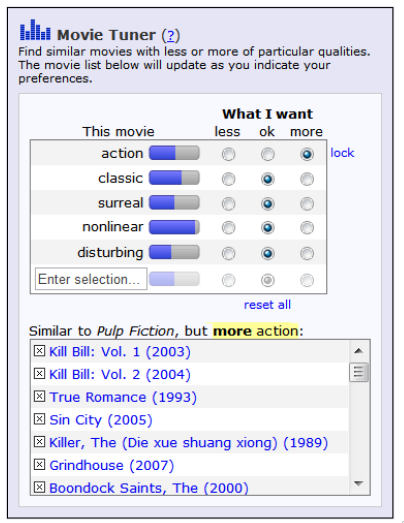
\includegraphics[width=0.7\textwidth]{graphics/stolenfigures/movietuner.png}
	\slcaption{
		The Movie-Tuner Interface from \cite{VISR12} %TODO: cite exact figure (" … as seen in [8, Fig. 33]")
		\label{fig:movietuner}}
\end{figure}

While the result of their algorithm aligns very much with the desired goal of this work, their implementation relies on supervised learning that requires a hand-labelled dataset.

\subsection{The algorithm of \textcite{Derrac2015}}

% Many \gls{cl} tasks rely on such knowledge bases, however generating them has occcupied scientists for dozens of years with only little significant progress, making its automatic creation an important achievement for the entire field.

To summarize, the kind of recommendation aimed for here would require a structured knowledge base that can be created from any domain in a data-driven way. This knowledge base can be represented as a vector space of human-interpretable, linearly independent components. A euclidian distance metric for the space would ease human interpretation. 

Famously, the idea of \textbf{Conceptual Spaces} fulfills these criteria. Introduced by Peter Gärdenfos in his 2000 book \citetitle{Gardenfors2000a} \cite{Gardenfors2000a} as a bridge between symbolic and subsymbolic processing, conceptual spaces represent knowledge in a geometric structure consisting of various quality dimensions. While well-known primarily as a theoretical model, an algorithm to automatically generate such spaces in a data-driven way was proposed by \textcite{Derrac2015} in 2015.

Their primary motivation is the following: Classical symbolistic AI relying on semantic knowledge bases can provide intuitive explanations for its decisions, but automatic creation of such has thus far been unsuccessful. Inspired by the way humans deal with incomplete knowledge, they draw a connection between commonsense reasoning patterns and the relation of concepts and entities in a conceptual space, claiming that qualitative spatial relations in the latter correspond to the semantic relations required for reasoning that help to fill gaps in these knowledge bases. In doing so, they create multiple classifiers that provide intuitive explanations for each decision. 

Given the widely accepted assumption that, algorithmically, recommendation is nothing beyond classification \cite{Linden2003,Ai2018,Sarwar2000}, \gencite{Derrac2015} algorithm seems the perfect base to allow for explainable recommendation as required here if it works reasonably well for the given domain.
%TODO: movie tuner doch schon eher einbringen und die connection ziehen "sowas wollen wir, aber data-driven, und Derrac2015 macht ebendas"?

Precise study of the pertinent literature has shown that there is a small but active community publishing improvements to this algorithm. However, most of these follow-up works include one of the authors of the primary paper, Steven Schockaert, as co-author \cite{Ager2018,Alshaikh2020}, indicating a small impact beyond this community. Furthermore, most of the considered literature use manually created datasets collected from multiple human reviews or tags, and given that the algorithm relies on the fact that relevant words occur more often in the text corpus, there is reason to assume that it may struggle when applied to the corpus given in this thesis. For these reasons it seemed reasonable to thoroughly test the domain transfer of the algorithm.

Unfortunately, the available open-source implementations that were found\footnote{\cite{Ager2018}: \url{https://github.com/ThomasAger/Autoencoder-Explanations}\\ \indent \phantom{\textsuperscript{10}} \cite{Alshaikh2020}: \url{https://github.com/rana-alshaikh/Hierarchical_Linear_Disentanglement}} proved undocumented and obscure,\footnote{Relying for example on 70 unnamed command-line arguments: \url{https://github.com/ThomasAger/Autoencoder-Explanations/blob/master/src/_archive/lr_pipeline.py\#L1211-L1283}}
 which is why it was decided that a complete re-implementation is the better idea and also less work. 

This also resulted in a new goal, namely, to create a reliable architecture for the algorithm that adheres to modern standards of software quality, as specified in \textbf{ISO/IEC 9126} and its replacement \textbf{ISO/IEC 25010:2011}, in the hope of making future research just like this one - where the validity of the algorithm and its ability to transfer to new domains is tested - easier than it was for \me.

% \includeMD{pandoc_generated_latex/1_1_motivation}


\section{Research Questions \& Thesis Goals}
% Goals of this work & Research-Questions
\label{sec:goals_research_questions}

In summary, the primary motivation for this thesis is to test if the methodology of \textcite{Derrac2015} is applicable to the domain of educational resources to find regularities in the data and allow for explainable recommendation of these. 

The methodology relies on many modular components with no obvious reason to choose any hyperparameter or component over another, resulting in a combinatorical explosion of runs, each with a significant runtime. Throughout the development of the respective code, the importance of a solid software-foundation became clear, leading to a shift in focus away from quickly generating results towards the methodology for a scalable, adaptable and qualitative architecture that may serve as foundation to answer many related research questions in the future. Among others, this includes the application of the algorithm to compute clusters such as the \gls{ikw} Grid Engine. The domain transfer to educational resources shall, however, still serve as prototypical application for which answers will be generated.

So, this thesis shall not only replicate the results of \cite{Derrac2015} and transfer their algorithm to a domain with practical benefits, but also deliver qualitative software for future research. To make this even easier, there will be a strong textual focus on the architecture as well, in the hope of allowing other scientists to work with this code-base. To show that the implemenation works, it will be also applied to an original dataset of \cite{Derrac2015} and the results will be compared.

\textbf{Clearly defined, the two stated goals of this thesis are thus:}

\begin{enumerate}
	\item Implement and describe a qualitative, scalable and adaptable software-architecture for the replicated algorithm, that can be used to easily apply it to new domains.
	\item Apply the methodology to the domain of educational resources to verify if the algorithm works and is useful to find regularities in the domain, allowing for explainable recommendation. In terms of original contributions, this includes finding differences in the structure of the given datasets and providing additions to the algorithm such that it works not only on specifically curated datasets.
\end{enumerate}

\subsection{Success conditions}

Exact evaluation metrics will be explained in detail later, but let us quickly define a few conditions that indicate successful execution of these goals.

\subsubsection*{Regarding the architecture}

A successful architecture is given if 

\begin{itemize}
	\item The results of \cite{Derrac2015} and its follow-up works \cite{Ager2018,Alshaikh2020} can be replicated for at least one of their original datasets
	\item The architecture sucessfully runs on the compute grid, indicating scalability and modularity.
	\item The criteria for software quality as specified in \textbf{ISO 25010} and open science are fulfilled.
	\item The code is open-sourced, well-documented and understandable.
\end{itemize}

\subsubsection*{Regarding the application of the algorithm to a new domain}

The main question to be answered here is \textit{Is the algorithm applicable for the domain of educational reasources}. This question must be explicitly answered by first stating the hypothesis, explainining the methods used, reporting results and subsequently discussing them. Unfortunately, the main success criterion of the algorithm is its subjective persuasiveness, which is hard to objectively and quantitatively evaluate without a study. For that reason, there is the need to find good surrogate metrics instead. Criteria for success include:

\begin{itemize}
	\item The difference from the given dataset to the originally used ones is elaborated and regarded for.
	\item Proper scientific methodology will be conducted for the evaluation of the results.
	\item The resulting semantic directions are \textit{convincing} in a sense that they fulfill demanded criteria that were specified before looking at results.
	\item The resuling semantic directions can be used as basis for explainable recommenders.
	\item These recommenders achieve similar performances to modern \gls{ml} techniques when applied to find human categories such as a course's faculty from the data.
\end{itemize}


% \includeMD{pandoc_generated_latex/1_2_thesisgoals}
